\documentclass[12pt]{article}
\usepackage{eurosym}
\usepackage[top=1in, bottom=1in, left=1in, right=1in]{geometry}
\usepackage{adjustbox}
\usepackage{amsmath}
\usepackage{amssymb}
\usepackage{array}
\usepackage{booktabs}
\usepackage{fancyhdr}
\usepackage{float}
\usepackage{graphicx}
\usepackage[colorlinks=true,linkcolor=blue,urlcolor=blue,anchorcolor=blue,citecolor=blue]{hyperref}
\usepackage{lscape}
\usepackage{multirow}
\usepackage{natbib}
\usepackage{setspace}
\usepackage{tabularx}
\usepackage[colorinlistoftodos,linecolor=black]{todonotes}
\usepackage{appendix}
\usepackage{pgffor}
\usepackage{adjustbox}

\parindent 22pt
\newcommand{\indep}{\rotatebox[origin=c]{90}{$\models$}}
\newcolumntype{L}[1]{>{\raggedright\arraybackslash}p{#1}}
\newcolumntype{C}[1]{>{\centering\arraybackslash}p{#1}}
\newcolumntype{R}[1]{>{\raggedleft\arraybackslash}p{#1}}
\begin{document}

\title{Analysis of the Reggio Approach}
\author{Pietro Biroli, Daniela Del Boca, and Chiara Pronzato}
\date{[VERY PRELIMINARY DRAFT] \\
Original version: January 22, 2016 \\
Current version: \today }
\maketitle

\bigskip

\doublespacing

\section{Introduction}\label{sec:intro}

This paper aims to evaluate the Reggio Approach preschool system. The Reggio Approach includes infant-toddler centers (ages 0-2) and preschools (ages 3-5), both of which are for children before they enter primary school at age 6. The Reggio infant-toddler center has a long history: it was established in 1971, while the first Reggio preschool was established even earlier, in 1963.

The Reggio Approach (RA) is a unique natural experiment which has been in place for fifty years in the city of Reggio Emilia, Italy. Here a universal high-quality early child care system has developed a more progressive vision of the child as an individual with rights and potential (\cite{Malaguzzi1993}). The Reggio Approach has received world-wide recognition and was defined as an exemplary model of early childhood education by Newsweek in 1971. It has received over the years several prizes and has been emulated in different countries,\footnote{The official \href{http://www.reggiochildren.it/network/?lang=en}{Reggio Children International Network} is present in 33 countries worldwide. Many other preschools around the world are ``inspired'' by the Reggio Approach but they are not officially part of these network.} but it has never been evaluated.

In order to evaluate the Reggio Approach, we have collected data on five age cohorts, three cohorts of adults, one cohort of adolescents, and one cohort of children in their first year of elementary school. The data were collected in Reggio Emilia, Padova, and Parma. Parma and Padova are similar to Reggio Emilia in several dimensions (size, geographic, demographic and socio-economic structure, and fertility dynamics), but do not provide the same type of early childhood education. The schools that follow the Reggio Approach are the municipal infant-toddler centers and preschools in Reggio Emilia. All of the children who attended a municipal infant-toddler center or preschool in Reggio Emilia are considered part of the treated group, since they received the RA intervention. The other types of schools in Reggio Emilia, and all the schools in Parma and Padova (including the municipal schools) did not receive the RA intervention.

Our analysis is limited to children and adolescents since the important outcomes collected in our survey are quite similar among them. Moreover these two cohorts are likely to have experienced similar childcare supply and choices. We are currently working on another section of the paper on the adult cohorts. They have faced very limited choice of formal childcare since the first experience started in the early sixties in Reggio Emilia and only later in the other two cities.

The evaluation of the Reggio Approach presents several challenges, given the non-experimental nature of the program. The RA preschool system was introduced and grew over the course of several decades; therefore the evaluation strategy has to deal with potential changes in treatment quality over time, lack of well defined control group, and potential spillover effects. This analysis evaluates the RA aiming to address these issues. We consider several groupings of controls to account for differences by region, data collection, socioeconomic factors, and most importantly type of preschool chosen by the families. Different model specifications allow for comparison with various control groups, allowing for a more nuanced understanding of the effects of RA, including the effects both within and between regions and in relation to other types of early education.

In the next section, we review some of the previous work on the impact of child care quality and curriculum on child outcomes. A brief description of the RA is provided in Section \ref{sec:RA} while a comparison between Reggio Emilia and the other two cities involved with the data collection is provided in Section \ref{sec:ParmaPadova}. More detail about the data collection, including sample structure and survey design, is given in Section \ref{sec:data}. A simple model of school selection is sketched in Section \ref{sec:model}. The identification strategy and the empirical analysis are discussed in Section \ref{sec:method}. Section (\ref{sec:conclusion}) provides very preliminary conclusions.

\bigskip

\section{The link between childcare quality, curriculum, and child outcomes} \label{sec:lit}

In the last few years economic research has started analyzing the impact of child care on child outcomes focusing not only on its availability but also its quality and pedagogical philosophies. \cite{Felfe2015a} analyzed German data, using information on the quality of available childcare for children under the age of three. They show that quality is a very important determinant of several child outcomes at the age of 6, particularly of socio-emotional maturity and school readiness. Specifically, teachers' age and education, working hours, and group size have a positive impact on child outcomes. The effects are stronger for children of less educated mothers.

\cite{Love2003} using data from three different contexts in the U.S., Australia, and Israel (Early Head Start; the Sydney Family Development Project; Haifa-NICHD merged data) compare a variety of childcare centers differing in levels of regulation and of staff quality, and provide consistent evidence that the quality of child care has an important impact on child development. In particular, children from low-income families experience a stronger positive impact of childcare quality on a both cognitive and non-cognitive outcomes.

\cite{Li2013} explore the effects on later outcomes of high-versus low-quality childcare both during infant--toddlerhood and during the preschool years, using data from the National Institute of Child Health and Human Development Study of Early Child Care. They show that quality matters as well as the timing of attendance of high-quality education. Cognitive, language, and other skills were highest in children who experienced high-quality care in both the infant--toddler and preschool periods, somewhat lower in children who experienced high-quality child care during only one of these periods, and lowest among children who experienced low-quality care during both periods.

Other studies have linked quality with the influence of certain program curricula and pedagogical philosophies on the teaching strategies employed in classrooms, roughly divided into the two main categories of ``child centered'' and ``academic'' approaches. The Reggio Approach is a clear example of a child centered approach, where the teacher is encouraged to become the child's co-learner and collaborator. According to this approach, teachers do not impose a specific curriculum, but facilitate the child's learning by planning activities based on the child's interests, and engaging in the activities alongside the child (\cite{Malaguzzi1993}, \cite{Hewett2001}). In an academic approach, instead, the focus is on acquiring notions related to different subject areas.

Using data from the Pre-K Survey of Beliefs and Practices, \cite{Marcon1999} identifies three different preschool models operating in an urban school district: child centered, academic driven, and a combination of the two. His empirical evidence shows that by the end of preschool, children from child-centered programs have acquired greater competence in social, basic math, and basic verbal skills than their peers in academically-driven preschool environments.

Other studies have compared the long term effects of several pedagogical models. \cite{Miller1984a} analyzes the achievement test and IQ data on low-income black youths who had participated in traditional and more progressive programs in preschool and prekindergarten through ninth and tenth grades. They find long-term positive effects of child-centered learning on school achievement. \cite{Schweinhart1997} have evaluated long term effects (through age 23) of the High/Scope program vs more traditional preschool curriculum models. Their findings show that using a curriculum model based on child-initiated learning activities improves social behavior at a later age. Specifically they found at age 23, compared to the other curriculum groups, the group who has experienced a more traditional curriculum had three times as many felony arrests per person.

The traditional sequential and subject specific approaches are less effective in promoting children's learning in the early years whereas a holistic approach that sustains children's overall development across several domains is more effective as it is supportive of children's learning strategies (\cite{Bennett2012}). As stated by \cite{Bennett2013}: ``The cognitive life of a young child does not match a traditional `subjects' approach. Rather, it is focused on meaning-making -- his/her place in the family; the roles and work of significant adults; forging a personal identity; how to communicate needs and desires; how to interact successfully and make friends; how things work; the change of the season and other remarkable events in the child's environment.''

While the RA has certainly a leadership role in promoting a child-centered approach and represents a long lasting pedagogical experience, these principles are increasingly becoming part of large number of child care experiences in different contexts in Italy as well as in other countries (\cite{Lazzari2012}).

\section{The Reggio Approach} \label{sec:RA}
% Quick description of Reggio Approach history
This section briefly describes the Reggio Approach.\footnote{For a more complete discussion of the Italian early childhood landscape and the educational philosophy of RA, see \citet{biroli2015evaluating}.} The Reggio Approach to early childhood education is a community effort of public investment in high-quality early childhood education spearheaded and led by the pedagogist Loris Malaguzzi (1920-1994), whose foresight has been the main influence on the approach. Since Malaguzzi became Pedagogical Consultant to Reggio Emilia municipal school in 1963, more and more progressive models of early childhood education characterized the municipal schools in Reggio Emilia previously dominated by Catholic traditional schools. The system evolved slowly over the years from a parent cooperative in the outskirts of Reggio Emilia into a structured municipal system of 26 infant-toddler centers and 30 preschools, in alternative to the prevailing Catholic schools which have declined rapidly after that.

Its education project built on existing pedagogical models combined with many innovative features. As stated by \cite{Edwards1993} this curriculum facilitates children's construction of their own powers of thinking through all the expressive, communicative, and cognitive languages.

The Reggio Children Approach views early childhood education as based on relationships, and focuses on each child in relation with other children, family, teachers, society and the environment. Its philosophy is based on several principles (\cite{Rinaldi2005,Gandini1993}).

First of all, children are seen as researchers: they develop theories and adapt them, individually and with others, while they interpret and reconstruct the world and their surroundings. These learning conditions are favored by the creation of small working groups of children and adults researching together. Collaborative group work is considered valuable and necessary to advance cognitive development. Children are encouraged to dialogue, compare, negotiate, and problem solve through group work.

Second, teachers are encouraged to facilitate the child's learning by planning activities and lessons based on the child's interests, asking questions to further understanding, and actively engaging in the activities alongside the child, as partners to the child more than only an instructor (\cite{Hewett2001}). According to the principles of RA, each class is organized with two teachers (often male and female), who are supported by a new professional figure, the ``atelierista'', a teacher trained to foster the children's expressive and creative languages.

Third, a continuous documentation of children's work in progress is constructed as an important tool for the learning process for children, teachers, and parents. Pictures of children engaged in experiences, their words as they discuss what they are doing, feeling and thinking, and the children's interpretation of experience through the visual media are displayed daily and used as assessment and memories. Other benefits of documentation include: making children's learning process visible, sharing their experiences with the parents, and allowing teachers to record and understand children learning dynamics.

A fourth important element concerns the teachers training. An ongoing and continuous job-training and collegial workplace for all educational figures is established, and it is deemed an integral part of the educational experience. Training is achieved through internal weekly updates, classroom teaching, and meetings that become a tool for dialogue, discussion, and growth among the various professional figures at the school.

Another important aspect concerns the space of the educational experience. Since the beginning, the aesthetic dimension was considered an integral part of learning, from the architecture, furniture, to the materials used in the school. The early municipal schools, opened in 1963 and 1964, were already equipped with an internal kitchen, and its personnel was actively involved in the educational project, an important and innovative choice for a public service. In each room there are mirrors (on the walls, floors, and ceilings), photographs, and children's work accompanied by transcriptions of their discussions. The environment has been defined by Malaguzzi the ``third teacher'' besides children and teachers.

Finally, parents are a vital component to the Reggio philosophy. They are viewed as partners, collaborators of their children's learning as they are involved in every aspect of the curriculum. Teachers conduct frequent meetings with parents to help educate them about children's social, emotional, creative and academic development. The educational project of early childhood is outcome of of the joint work of teachers, pedagogists, and parents in Consigli Infanzia Citt\`{a} (City Infant Councils) which are elected every three years.

In the next sections we will try to analyze differences and similarities in Reggio Emilia, Parma, and Padova in order to understand and interpret better our empirical results.

\section{Reggio, Parma, and Padova} \label{sec:ParmaPadova}

% Reggio Emilia vs. Parma vs. Padova
In addition to collecting data from individuals in Reggio Emilia, data were collected from individuals in Parma and Padova, two cities that share several features with Reggio Emilia. %Table (\ref{tab:comparison}) lists some characteristics of the three cities.
More information on the data collection is given in Section (\ref{sec:data}).

While in the rest of the paper we will show several similarities between Reggio Emilia, Padova and Parma concerning size, geographic, demographic, and socio-economic structure, in this part we discuss some of the differences concerning the pedagogical approach and infant-toddler centres' and preschools' organization (children and teachers' roles,documentation, type of training, parental involvement, environment etc) in the three educational systems.

%\begin{table}[ht]
%\caption{Demographic Comparison of Reggio Emilia, Parma, and Padova}
%\label{tab:comparison}
%\begin{center}
%\begin{tabular}{lccc}
%\hline\hline
%& \multicolumn{3}{c}{City} \\ 
%\cmidrule{2-4} & Reggio Emilia & Parma & Padova \\ \hline
%Population (2013)* & 172,525 & 187,938 & 209,678 \\ 
%Average per-capita income (2011 euros)** & 25,226 & 28,437 & 29,915 \\ \hline
%\end{tabular}
%\end{center}
%\par
%{\footnotesize Notes: *ISTAT, \url{http://www.demo.istat.it/}; **Finance Minister, taxable income for 2011. }
%\end{table}
%%\todo[backgroundcolor=orange!30,size=\tiny]{Add the information collected by Linor}

First of all, the Reggio Emilia municipal infant-toddler centers and preschools are certainly the oldest childcare system in Italy: it started in 1963 with the opening of the first municipal preschool, and in 1971 with the opening of the first municipal infant-toddler center, earlier than the 1971 National Law. Municipal schools in Padova (1976-77) and Parma (1975) instead started after the law, in the mid-late seventies.

% Preschool availability and take-up

% Different types of preschool
As in every Italian city, early educational experiences are divided into two main age categories. The first, infant-toddler centers (asilo nido), is available for children aged 0 through 3 while the second, preschool (scuola materna/dell'infanzia), is for children aged 3 through 6.

For each of these age groups, there are schools established and managed by different entities: municipal, state, private, and religious. Table \ref{tab:types} summarizes the types of schools available for each age group, highlighting that there are no state-run infant-toddler centers.

\begin{table}[ht]
\caption{Types of Schools}
\label{tab:types}
\begin{center}
\begin{tabular}{ccc}
\hline\hline
& Infant-Toddler & Preschool \\ \hline
Municipal & \checkmark & \checkmark \\ 
State &  & \checkmark \\ 
Private & \checkmark & \checkmark \\ 
Religious & \checkmark & \checkmark \\ \hline
\end{tabular}
\end{center}
\end{table}

The schools that follow the Reggio Approach are the municipal infant-toddler centers and preschools in Reggio Emilia. All of the children who attended a municipal infant-toddler center or preschool in Reggio Emilia are considered part of the treated group, since they received the RA intervention. The other types of schools in Reggio Emilia, and all the schools in Parma and Padova (including the municipal schools) did not receive the RA intervention.

In Italy, early childhood education is provided at the public level (State and Municipal) and by private organizations (religious and secular private companis). The system is decentralized: the municipality is the main decision-maker, while the regions define general management criteria;\footnote{To date, in Italy there are 8,092 municipalities in 101 provinces and 20 regions.} The central government is only responsible for defining common objective standards and resources allocation among regions (\cite{Brilli2016}).

Two Italian laws regulate the provision of early childhood services. Enacted in 1968, the law 444 provided for state-run preschools (target at ages 3 to 5) and enabled municipalities to create their own autonomous early childhood programming. This law assigned the costs of building, equipment, and playing materials to the State; municipalities were to fund building maintenance, heating, and operating costs including salaries for an all-female staff of teachers under 35 years of age with a high school diploma. The second one, Law 1044 enadacted in 1971, mandates regional governments to construct and operate enough infant-toddler centers (asili nido) to meet the local demand for childcare for children aged 3 to 36 months (\cite{Brilli2016}).

Municipalities have been also enabled to set eligibility criteria giving preferential access to whom public childcare appears to be most valuable. Selection criteria appear to be similar across municipalities, however the weighting of distinct family characteristics varies. In the last decade, childcare supply from private providers has increased and developed differently across Italian regions (Istituto Degli Innocenti, 2002 and 2009). Public childcare differs from private childcare in several ways. For instance, public services are more strictly regulated both in terms of service standards and in terms of management and personnel requirements (Istituto Degli Innocenti, 2002). As recently stated in Budget Law 2002,\footnote{Law 448/2001 (Budget Law 2002) defined formal childcare as ``structures aimed at granting the development and socialization of girls and boys aged between 3 months and 3 years and to support families and parents with young children.''} one of the most important aim of public childcare is educational. This goal has been implemented through the introduction of quality standards, especially in regions with greater experience in childcare provision, such as Emilia Romagna and Tuscany. Public childcare is also less expensive than the private one, since it is highly subsidized for lower income families.

The Italian child care quality is relatively high compared to other countries. According to the European ranking, Italian public child care it is fourth after Denmark, Finland, and France (\cite{DeHenau2008}).

While high quality standards are common among public schools, there is still variation in the curriculum across municipalities and regions.

In this section we aim to compare Reggio Emilia to Parma and Padova. While the first two are both provinces of Emilia Romagna, a region with a long standing left-leaning tradition in public administration, Padova is a province of Veneto, traditionally a very Catholic region and a long time stronghold of the centrist political party Christian Democracy.

In Padova, the pedagogical approach is influenced by Frabboni (\cite{Frabboni1999}) and is based on a more traditional cognitive child approach, that is not child-centered as RA. The presence of a large number of religious schools still have potential strong spillovers on the philosophy of the municipal childcare. \textbf{(CITE)}

Differently from RA, teachers have a more traditional role as instructors who follow a sequential and academic program and there is no role for a teacher with specific art and creative skills to stimulate and coordinate children's activities.

Similar to RA, also in Padova's municipal schools teachers document the activities and collect materials produced by teachers and children. However, this is done ex-post and used as a archive for valuation of children's work and communication with the parents \footnote{See Piano dell Offerta Formativa of preschools and nidi in Padova 2016 \url{http://www.padovanet.it/sites/default/files/attachment/Progetto\%20pedagogico.pdf}} Teachers undergo frequent training, but unlike in RA this is not a continous process but is scheduled at specific times and is provided in classroom with traditional lecture format.

Parents are informed about the children activities and progress in specific meetings. Teachers undergo frequent training, but unlike in RA this happens at specific times and is provided in classroom with traditional lecture format. Finally most schools have their own kitchen, but food is often provided by an external company. 

Parma as Reggio Emilia is a province of Emilia Romagna, a region which forms the famous Italian ``Red Quadrilateral'' with Tuscany, Umbria and Marche. The left-wing tradition is due to the strength of the anti-fascist resistance around the time of World War II as well as a strong history of anti-clericalism dating from the 19th century, when part of the region belonged to the Papal States. However the political history of Parma has been different from Reggio Emilia. During the period 1950-1990 a moderate socialist party has been predominant and afterwards the center-right has controlled the city administration. In Parma, the pedagogical approach is not based on a unique pedagogical approach, but is influenced by a combination of different ones.\footnote{The summary of the pedagogical approach in Parma is based on \cite{Parma2006} and an interview with Rossana Allegri, responsible for the municipality of Parma for the management of preschools. From these documents and informal interviews with coordinators of servizi educativi of Parma and Padova and Reggio Emilia, it looks the curriculum in Parma is a combination of Padova and Reggio Emilia.} Among others \cite{Winnicott1965} and \cite{Bion1962} who have stressed the importance of the mother-child link which required a very long and articulated adjustment period for the child to be separated from his/her family to attend child care.

According to the Piano dell' Offerta Formativa of infant-toddler centres and preschools (2016), ``children should have a central role in the learning process which allows to achieve a dimension of knowledge not as a performance, but as opportunity of supporting independent and original building of his/her personality.'' In spite of some similarities with RA in the role of children and teachers, in Parma there is no role for a teacher coordinator with a creative and artistic background (atelierista).\footnote{See \url{http://www.comune.parma.it/servizieducativi/it-IT/Servizi educativi}} 

Parents can intervene in the schools'life with ideas proposals and experiences but are not intgral part of the curriculum.

Training are not continous but provided at specific times. There is an informal traing which consists in meetings with the pedagogical coordinator and a formal training which is provided in classroom with traditional lecture format by university professors.

Finally, important differences characterize also the organization of child care (see \cite{DelBoca2016}). The eligibility criteria in Padova is mainly geographical, while in Parma priority is given to families in difficulty (health issues and single parent families) as well as parental working hours, similarly to Reggio \citep{Frabboni1999}.

In summary, the early childhood education provision in both Parma and Padova presents some similar features to the one of Reggio Emilia: schools have good quality of care, and their teaching and educational philosophy is based on respected developmental principles which evolved in symbiosis with the Reggio Approach. However, as discussed above a few features are partially different. These similiarities and differences have to be taken into account in the interpretation of our results.


\section{Data}
\label{sec:data}

This section discusses the survey data which has been used for the analysis in this report.\footnote{Also administrative data from the RA preschool system was collected. Its description and more details about the survey data are contained in \citet{biroli2015evaluating}} To evaluate the impact of Reggio, individuals living in Reggio Emilia, Parma, and Padova since their first year of life were interviewed. Data were collected on five age cohorts, including three cohorts of adults, one cohort of adolescents, and one cohort of children in their first year of elementary school.

The structure of the cohorts is described in Table \ref{tab:cohorts}.

\begin{table}[ht]
\caption{Cohort Structure}
\label{tab:cohorts}
\begin{center}
\begin{tabular}{ccc}
\hline\hline
Cohort & Years of Birth & Age at Interview \\ \hline
I & 1954--1959 & 54--60 \\ 
II & 1969--1970 & 43 \\ 
III & 1980--1981 & 32 \\ 
IV & 1994 & 18 \\ 
V & 2006 & 6 \\ \hline
\end{tabular}
\end{center}
\end{table}

%In order to fix ideas on the identification strategy, we currently focus our attention only on the adolescents, the cohort for which we have the most wide array of information on both the caregiver and the respondent of interest.\textbf{I would add all cohorts in this table to show that different cohorts have different options of school types}


Table (\ref{tab:sample-adol}) and Figures (\ref{fig:asiloAttend}-\ref{fig:preschoolAttend}) show the number of children, adolescents, and adults interviewed in our sample who attended the different types of child-care in Reggio Emilia, Parma, and Padova.\footnote{Note that these percentages are not necessarily representative of the whole populations of the cities, since participants to the Reggio Approach were slightly oversampled in order to reach at least 150 participants who attended either RA infant-toddler centers or RA preschool in each Cohort. See \citep{Biroli2015} for more details.}

\begin{table}[ht]
\caption{Sample Size by City and School Type; Children and Adolescents}
\label{tab:sample-adol}
%tab asiloType City if Cohort==1
%tab maternaType City if Cohort==1
%tab asiloType City if Cohort==3
%tab maternaType City if Cohort==3

\begin{center}
\begin{tabular}{l ccc|ccc}
\hline\hline
 & \multicolumn{6}{c}{\textit{\textbf{Children born in 2006}}} \\ 
 & \multicolumn{3}{c}{\textit{Infant-Toddler Center}} & \multicolumn{3}{c}{\textit{Preschool}} \\ 
 & Reggio & Parma & Padova & Reggio & Parma & Padova \\ \hline
Not Attended    & 117 &  98 & 143 &   2 &   6 &   2 \\ 
Municipal       & 160 & 149 &  68 & 166 & 154 &  82 \\ 
State           &   . &   . &   . &  45 &  43 &  40 \\ 
Religious       &  27 &   7 &  26 &  92 &  77 & 141 \\ 
Private         &   6 &  36 &  41 &   5 &   9 &  12 \\ \hline 
%
%
\rule{0pt}{1.2\normalbaselineskip}
 & \multicolumn{6}{c}{\textit{\textbf{Adolescents born in 1994}}} \\ 

 & \multicolumn{3}{c}{\textit{Infant-Toddler Center}} & \multicolumn{3}{c}{\textit{Preschool}} \\ 

 & Reggio & Parma & Padova & Reggio & Parma & Padova \\ \hline
Not Attended    & 130 & 130 & 210 &   7 &   4 &   1 \\ 
Municipal       & 153 &  97 &  61 & 116 & 116 &  93 \\ 



State           &   . &   . &   . &  22 &  43 &  47 \\ 
Religious       &   9 &  10 &   8 &  96 &  82 & 131 \\ 
Private         &   3 &  13 &   0 &   6 &   6 &   6 \\ \hline
%
%
\rule{0pt}{1.2\normalbaselineskip}
 & \multicolumn{6}{c}{\textit{\textbf{Adults born in 1980-1981}}} \\ 
 & \multicolumn{3}{c}{\textit{Infant-Toddler Center}} & \multicolumn{3}{c}{\textit{Preschool}} \\ 
 & Reggio & Parma & Padova & Reggio & Parma & Padova \\ \hline
Not Attended    & 211 & 192 & 222 &  57 &  44 &  47 \\ 
Municipal       & 60  &  40 &  19 & 149 &  98 &  35 \\ 
State           &   . &   . &   . &  31 &  51 &  26 \\ 
Religious       &   3 &   8 &   5 &  40 &  50 & 140 \\ 
Private         &   3 &  10 &   3 &   1 &   5 &   1 \\ \hline
%
%
\rule{0pt}{1.2\normalbaselineskip}
 & \multicolumn{6}{c}{\textit{\textbf{Adults born in 1969-70}}} \\ 
 & \multicolumn{3}{c}{\textit{Infant-Toddler Center}} & \multicolumn{3}{c}{\textit{Preschool}} \\ 
 & Reggio & Parma & Padova & Reggio & Parma & Padova \\ \hline
Not Attended    & 244 & 226 & 226 &  80 & 116 &  75 \\ 
Municipal       & 36  &  24 &  19 & 128 &  52 &  27 \\ 
State           &   . &   . &   . &  17 &  26 &  24 \\ 
Religious       &   0 &   3 &   7 &  52 &  55 & 123 \\ 
Private         &   0 &   1 &   0 &   5 &   1 &   0 \\ \hline
%
%
\rule{0pt}{1.2\normalbaselineskip}
 & \multicolumn{6}{c}{\textit{\textbf{Adults born in 1954-59}}} \\ 
 & \multicolumn{3}{c}{\textit{Infant-Toddler Center}} & \multicolumn{3}{c}{\textit{Preschool}} \\ 
 & Reggio & Parma & Padova & Reggio & Parma & Padova \\ \hline
Not Attended    & 198 &  86 & 138 & 147 &  72 &  57 \\ 
Municipal       &  0  &  13 &   0 &   9 &  12 &  11 \\ 
State           &   . &   . &   . &  10 &   7 &   2 \\ 
Religious       &   1 &   4 &   6 &  28 &  11 &  68 \\ 
Private         &   0 &   0 &   0 &   2 &   0 &   2 \\ \hline
\end{tabular}
\end{center}
\raggedright{\footnotesize {{\bfseries Notes:} Source: authors' calculations from  the survey data. Type of preschool derived from parental section of the children and adolescent questionnaires providing type, name and address of childcare attended. Those who reported not to attend were either in other forms of childcare (e.g. nanny), or at home.} }
\end{table}











\begin{figure}[!htb]
\caption{Type of Infant-toddler center attended, by city and cohort}
\label{fig:asiloAttend}
\begin{center}
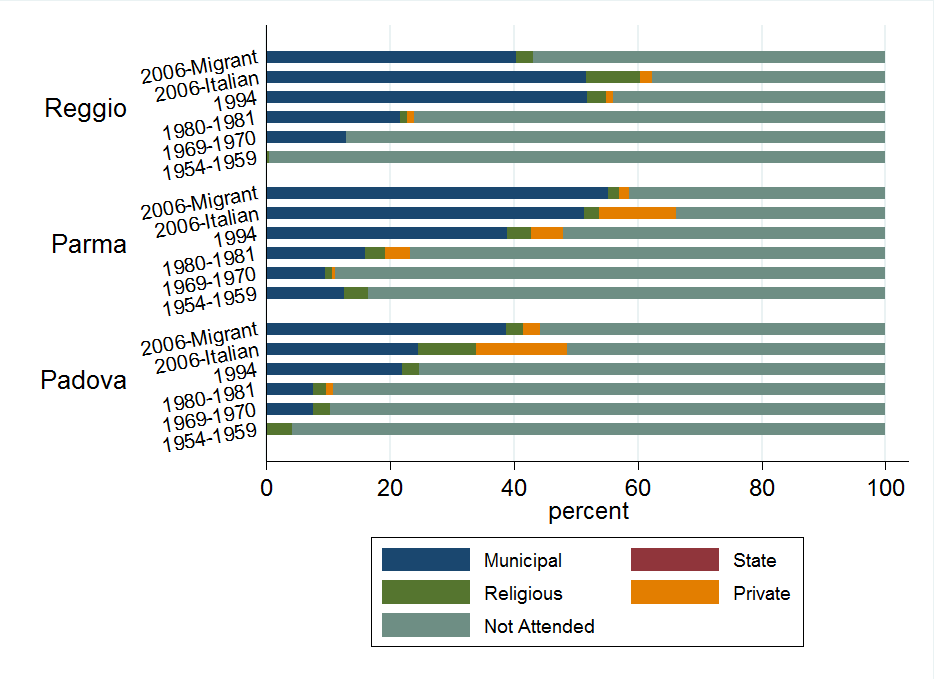
\includegraphics[height=8cm]{asiloType-Attend.png} \\[0pt]
\end{center}
\par
{\footnotesize {{\bfseries Notes:} Source: authors' calculations from the survey data. Type of infant-toddler center derived from parental section of the children and adolescent questionnaires providing type, name and address of childcare attended. Those who reported not to attend were either in other forms of childcare (e.g. nanny), or at home. It.=Italian. Imm.=Immigrant.} }
\end{figure}

\begin{figure}[!htb]
\caption{Type of Preschool attended, by city and cohort}
\label{fig:preschoolAttend}
\begin{center}
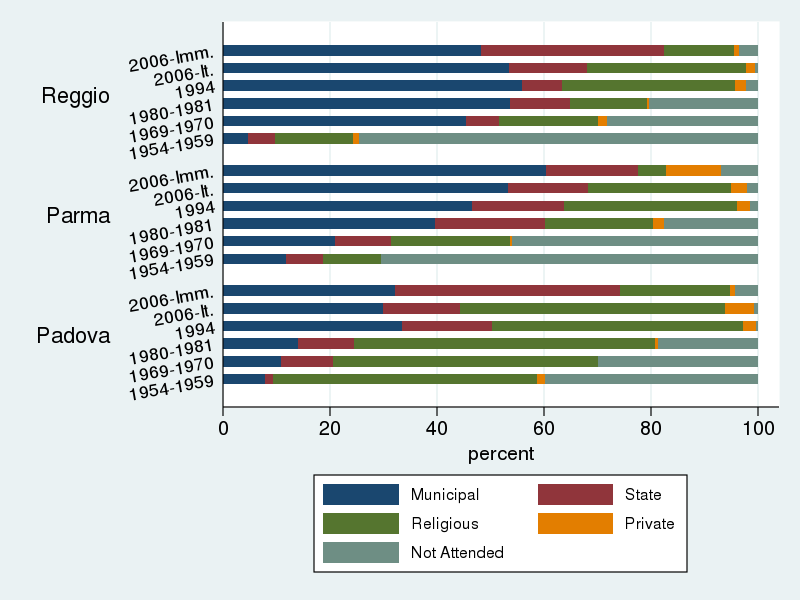
\includegraphics[height=8cm]{maternaType-Attend.png}\\[0pt]
\end{center}
\par
{\footnotesize {{\bfseries Notes:} Source: authors' calculations from  the survey data. Type of preschool derived from parental section of the children and adolescent questionnaires providing type, name and address of childcare attended. Those who reported not to attend were either in other forms of childcare (e.g. nanny), or at home. It.=Italian. Imm.=Immigrant.} }
\end{figure}

As we can see from the data, the distribution of school type is quite different across cities and over the different cohorts. First of all, we can see that participation in preschool and, later on, also infant-toddler centers increased over time for all the three cities. Furthermore, when comparing across the type of preschool, municipal infant-toddler centers and preschools are more popular in both Reggio Emilia and Parma, while Religious centers are predominant in Padova.\footnote{Again, note that these numbers are not necessarily representative of these cities and cohorts, but merely reflect our sample size, with an over sampling of municipal centers in the city of Reggio Emilia.} Private childcare centers entered the market later, and represent a very small share of respondents.

%%-------------------- Theoretical Approach ----------------------------------------------%
\section{Model of School Selection (Sketch)}
\label{sec:model}

In this section we sketch a theoretical framework which helps motivate and interpret our empirical results. In order to better understand the family decision to send the child to a Reggio Approach (RA) childcare center, consider a generalized Roy model framework. $Y_{1,i}$ represents the potential outcome of the child $i$ when attending an RA center, and $Y_{0,i}$ the potential outcome of the child when not attending an RA center. Define potential outcomes as follows:
\begin{align}
Y_{1,i}& =\beta_{1}(X_{i})+\varepsilon_{1,i} \nonumber \\
Y_{0,i}& =\beta_{0}(X_{i})+\varepsilon_{0,i} \nonumber \\
Y_{i} =& R_{i}Y_{1,i} + (1-R_{i}) Y_{1,i} \label{eq:outcome}
\end{align}%
where $\beta_{R}(X_{i})=E(Y_{R,i}|X=x)$ for $R=0,1$. The individual return to attending a Reggio Approach childcare center can be defined as the difference between these two potential outcomes, $\Delta_{i}^{RA}=Y_{1,i}-Y_{0,i}=\beta_{1}(X_{i})-\beta_{0}(X_{i})+\varepsilon_{1,i}-\varepsilon_{0,i}$.

The total costs of attending different types of preschools will systematically differ as well. First of all because public child care is subsidized in Italy, and therefore the fees charged by municipal, state, and religious schools vary according to family income. %\todo[backgroundcolor=orange!30,size=\tiny]{Insert table about fees, either here or in the appendix}
Secondly, because each family might face a different disutility costs of sending a child to a particular type of school, depending on the family background or the distance to the different schools. 
Let the costs associated with attending or not an RA childcare center for family $i$ be given by:
\begin{equation*}
V_{R}(X_{i},Z_{i})=\gamma_{R}(X_{i},Z_{i})+\eta_{R,i},\ R=0,1,
\end{equation*}%
where $X_{i},Z_{i}$ are observable characteristics of household $i$, and $EV_{R}(X_{i},Z_{i})=\gamma_{R}(X_{i},Z_{i}).$

Finally, the probability of attending an RA center will joint depend on the supply and demand of childcare slots, that is on the family decision of demanding a spot $R_{d,i}=1$, and the likelihood of getting accepted $R_{s,i}=1$. 
A family will choose to demand a slot in a Reggio Approach center when facing a positive perceived net benefit, $R_{d,i}=1 \Leftrightarrow I_{R,i} \geq 0$:

\begin{eqnarray*}
I_{R_{d,i}} &=&\left(Y_{1,i}-V_{1,i}\right)-\left(Y_{0,i}-V_{0,i}\right) \geq 0 \\

%&=&\left(\beta_{1}(X_{i})-\beta_{0}(X_{i})+\varepsilon_{1,i}-\varepsilon_{0,i}\right)-\left(\gamma_{1}(X_{i},Z_{i})-\gamma_{0}(X_{i},Z_{i})+\eta_{1,i}-\eta_{0,i}\right) \\
&=&\beta_{1}(X_{i})-\beta_{0}(X_{i})-\gamma_{1}(X_{i},Z_{d,i})+\gamma_{0}(X_{i},Z_{d,i})-\omega_{d,i} \geq 0 
%\\ &=& h(X_{i},Z_{d,i}) \geq W_{i}
\end{eqnarray*}%
which is determined by the family observable characteristics $X_{i},Z_{d,i}$ and their unobservables $\omega_{d,i} \equiv \varepsilon_{0,i}-\varepsilon_{1,i}+\eta_{1,i}-\eta_{0,i}$. %and the net systematic return of demanding a slot in a RA center can be represented as $R_{d}(X_{i},Z_{d,i})=\beta_{d}(X_{i})-\gamma_{d}(X_{i},Z_{i})$. 
On the other hand, since the past decades have seen an excess of demand, priority access to public childcare slots was given according to very specific observable criteria $R_{s,i}=R_{s,i}(X_{i},Z_{s,i})$, which were publicly known and commonly decided in the city of Reggio Emilia.\footnote{See section (\ref{sec:ParmaPadova}) as well as \cite{Brilli2016} for more details}. %\todo[backgroundcolor=orange!30,size=\tiny]{More deatails about access}

Assuming linearity of the $\beta_{R}(\cdot)$ and $\gamma_{R}(\cdot)$ functions, the probability of household $i$ attending RA will depend on the following system of supply and demand equations:
%
\begin{align}
R_{s,i} = & \gamma_{s} \left( Z_{s,i}, X_{i} \right) + \omega_{s,i}  \label{eq:1stage-supply} \\

R_{d,i} = & \gamma_{d} \left( Z_{d,i}, X_{i} \right) + \omega_{d,i}  \label{eq:1stage-demand} 

%
%R_{s,i} = & \gamma_{z_{s}} Z_{s,i} + \gamma_{x_{s}} X_{i} + \omega_{s,i}  \label{eq:1stage-supply} \\
%R_{d,i} = & \gamma_{z_{d}} Z_{d,i} + \gamma_{x_{d}} X_{i} + \omega_{d,i}  \label{eq:1stage-demand} 
\end{align}
%
such that we will observe a child attending a RA center $R_{i}=1$ if and only if they apply $R_{d,i}=1$ and get accepted $R_{s,i}=1$.
Note that the observables $Z_{s,i}$ and $Z_{d,i}$ are those characteristics of the household that shift the supply or the demand of childcare, but do not affect the potential academic and non-academic benefits of attending the two types of school. That is, the difference in attendance likelihoods for household $i$ are a function of the $X_{i}$ and $Z_{s,i},Z_{d,i}$ but the difference in school benefits between an RA school and a non-RA school are functions only of the observable characteristics $X_{i}$.

\bigskip

The variables observable to the econometrician are $R_{i},Y_{i},X_{i},$ and $Z_{s,i},Z_{d,i}$. Then we have the following system of equations:%
\begin{align}
E(R_{i}|X,Z)        =&  \gamma \left( Z_{s,i}, Z_{d,i}, X_{i} \right) + \omega_{i}  \label{eq:1stage} \\

E(Y_{i} |X,R_{i})   =& R_{i} E(Y_{1,i}| R_{i}) + (1-R_{i}) E(Y_{0,i}| R_{i}) \nonumber \\

   %=& R_{i} E\left(\beta_{1}(X_{i})+\varepsilon_{1,i} | R_{i}\right) + (1-R_{i}) E \left(\beta_{0}(X_{i})+\varepsilon_{0,i} | R_{i}\right)  \nonumber \\
   %=& \beta_{0}(X_{i}) + R_{i} \left(\beta_{1}(X_{i}) - \beta_{0}(X_{i}) \right) + E(\varepsilon_{0,i}| R_{i})  + R_{i} E \left(\varepsilon_{1,i}  - \varepsilon_{0,i} | R_{i} \right) \nonumber \\
   =& \beta(X_{i}) + \delta R_{i} + E(\varepsilon_{R,i}| R_{i}) \label{eq:heckit}

\end{align}
where we have made the simplifying assumptions that $\beta_{1}(X_{i})=\beta_{0}(X_{i})=\beta(X_{i})$ up to differences in a constant $\delta$ which captures the average effect of attending an RA childcare center, and $\varepsilon_{R,i} \equiv \varepsilon_{0,i} +R_{i} (\varepsilon_{1,i}-\varepsilon_{0,i})$.
Now assume that all of the disturbance terms in the model are distributed as a multivariate normal. Then $\varepsilon_{R,i}, \omega_{i}$ are normally distributed, and the conditional expectation $E(\varepsilon_{R,i}|R_{i})$ in (\ref{eq:heckit}) can be consistently estimated (up to a scalar constant) from a first stage probit, as in \cite{Heckman1979}. We can then estimate the regression function with the estimated (up to scale) value $E(\varepsilon_{R,i}|R_{i}),$ and this enables identification of $\beta,\delta$ and a small set of elements of the covariance matrix of $W_{i}.$ More efficient estimates of the identified parameters can be obtained through joint estimation of the $R_{i}$ and $Y_{R,i}$ dependent variables.

%
%%--------------------   Empirical Approach ----------------------------------------------%

\section{Empirical Methods} \label{sec:method}

In order to evaluate the effect of Reggio Approach childcare centers on individual outcomes we adopt different econometric methodologies and different sub-samples of our data.

In term of methodology, we initially estimate the parameter $\hat{\delta}$ in equation (\ref{eq:heckit}) using Ordinary Least Squares; we then estimate the system of equations (\ref{eq:1stage}-\ref{eq:heckit}) using an Instrumental Variable approach, and two types of Propensity Score Matching; finally, we use a differences-in-differences strategy comparing Reggio Emilia with the other two control cities.




In terms of sub-samples, the data contains information on respondents from the city of Reggio Emilia, where some children were treated and some were not, and in the two control cities of Parma and Padova, where all children were untreated. The first sub-sample is composed of children in Reggio Emilia only. The identification strategy rests on the idea that, although all children could apply for a slot in the RA childcare, some were more likely to apply and obtain a slot due to some exogenous factors. The second sub-sample is composed of treated children in Reggio Emilia and all children in Parma and Padova. The underlying idea is that some children in Parma and Padova were very similar to treated children in Reggio Emilia, but were not treated simply because there were no RA centers in their city. The final two sub-sample leverage the differences between the two control cities of Parma and Padova, comparing children who attended municipal and non-municipal childcare in the cities of Reggio Emilia versus Parma, and children in Reggio Emilia versus Padova. The idea rests on the fact that, although parents may have had unobservable preferences to select a particular type of school instead of another, the effect of RA can be recovered under the assumption that the selection was similar across the different cities.

Here below we describe the ten specifications used to evaluate the impact of RA childcare centers, the results of which are reported in tables (\ref{tab:childIT}-\ref{tab:adoPS}) below. For each outcome $Y_{i}$ two parallel analysis are carried out: one estimating the effect of attending an RA infant-toddler center during ages 0-3, and another focusing on the effect of attending an RA preschool during ages 3-6.

\subsection{Reggio Emilia Only}

Focusing only on the respondents from Reggio Emilia, we first estimate with OLS the following linearisation of equation (\ref{eq:heckit}):
\begin{equation}
Y_{i} = \delta R_{i} + \alpha_{C} C_{i} + \beta X_{i} + \varepsilon_{i}    \hspace{2ex} \text{ if } i \in \text{Reggio Emilia} \label{eq1:OLSreggio}
\end{equation}

where $Y$ is the outcome of interest, the dummy variable $C_{i}$ indicates whether the child attended any type of childcare center, $R_{i}$ whether he attended a Reggio Approach infant-toddler center, and $X_{i}$ represents the vector of predetermined control variables (age and gender of the individual, health at birth, family structure, parental educational and economic resources, house property, religiosity, and distance from the town center).\footnote{For simplicity, we use `she' to refer to the mother, and `he' to refer to child, although we consider both genders in the regressions.} $\delta$ and $\alpha_{c}, \beta,$ are the parameters to be estimated, while only the parameter of interest $\hat{\delta}$ will be shown in the tables of results. If there is no systematic selection into RA centers, such that $E(\varepsilon|R=1)=E(\varepsilon|R=0)=E(\varepsilon)$, then OLS estimation of $\hat{\delta}$ in equation (\ref{eq1:OLSreggio}) measures the additional effect of attending a RA center rather than any other childcare center in Reggio Emilia.

\medskip

Worried about potential selection into RA given by the endogeneity of parental childcare decisions, we estimate the system of equations (\ref{eq:1stage}-\ref{eq:heckit}) instrumenting the RA dummy with variables $Z$ related to distance between the house and the closest RA childcare center, the score the child would have got if applying to an RA childcare center, mother's place of birth and whether she attended a childcare center when young:

\begin{align}
R_{i} =& \gamma_{z} Z_{i} + \gamma_{x} X_{i} + \omega_{i} \hspace{2ex} \text{ if } i \in \text{Reggio Emilia} \label{eq:est1stage} \\

Y_{i} =& \delta \hat{R_{i}} + \alpha_{C} C_{i} + \beta X_{i} + \varepsilon_{i} \hspace{2ex} \text{ if } i \in \text{Reggio Emilia} \label{eq2:IVreggio}


\end{align}

\medskip

As third specification, we adopt a control function strategy. We first estimate the probability to attend a RA infant-toddler center as in (\ref{eq:est1stage}) and then include in (\ref{eq1:OLSreggio}) a third degree polynomial of the difference between the actual RA choice and the RA predicted probability:%\footnote{We experimented with different degrees of polynomial without substantial differences in the results.}

\begin{equation}
Y_{i} = \delta \hat{R_{i}} + \alpha_{C} C_{i} + \beta X_{i} + \sum_p \theta_{p} \left(RA_{i} - \widehat{RA_{i}} \right)^{p} + \varepsilon_{i} \hspace{2ex} \text{ if } i \in \text{Reggio Emilia} \label{eq3:CFreggio}
\end{equation}

Results from (\ref{eq2:IVreggio}) and (\ref{eq3:CFreggio}) are valid under the assumption that the instruments are correlated with the RA choice but not with the outcome of interest.

\subsection{Treated in Reggio Emilia, control in Parma and Padova}

As a fourth specification, we again estimate using OLS equation (\ref{eq:heckit}), however this time we limit the sample to those children who attended an RA center, or those living in Parma or Padova, so that the parameter of interest is estimated as the additional effect of attending a RA infant-toddler in Reggio rather than any other infant-toddler center in Parma and Padova:
%
\begin{equation}
Y_{i} = \delta R_{i} + \alpha_{C} C_{i} + \beta X_{i} + \varepsilon_{i}    \hspace{2ex} \text{ if } i \in \{\text{RA } \cup \text{ Parma } \cup \text{ Padova } \} \label{eq4:OLSrpp}
\end{equation} 

\medskip

As a fifth specification, in order to better approximate the observable characteristics of children in Parma and Padova who might have attended a RA center if only they were born in Reggio Emilia, we consider a Propensity Score Matching (PSM) approach. 
We apply to (\ref{eq4:OLSrpp}) probabilistic weights so that untreated children in Parma and Padova look similar -- considering weighted averages -- to treated children in Reggio Emilia. 
Probabilistic weights are calculated as:%
\begin{equation}
\left\{
\begin{tabular}{cl}
$\frac{1}{\widehat{R_{i}}}$   & if the child attended a RA school \\
$\frac{1}{1-\widehat{R_{i}}}$ & if the child did not attend a RA school
\end{tabular}
\right. \label{eq:weights}
\end{equation}
%
where the predicted probability of attending an RA center, $\widehat{R_{i}}$, is always obtained by equation (\ref{eq:est1stage}), estimated using only observations from Reggio Emilia.

\medskip

As a sixth specification, we take into consideration the fact that different observable characteristics drive the probability of demanding a slot in an RA center, and the probability of being accepted, as described in the system of equations (\ref{eq:1stage-supply}-\ref{eq:1stage-demand}).

Probabilistic weights in this specification are calculated as:
%
\[
\left\{
\begin{tabular}{cl}
$\frac{1}{ \widehat{R_{d,i}} \times \widehat{R_{s,i}}}$   & if the child attended a RA school \\
$\frac{1}{1-\widehat{R_{d,i}}  \times \widehat{R_{s,i}}}$ & if the child did not attend a RA school
\end{tabular}
\right.

\]
%
where $\widehat{R_{d,i}}$ is the estimated probability of demanding a RA childcare slot, and $\widehat{R_{s,i}}$ is the estimated probability of being offered a RA slot. These probabilites are estimated using a partial observability model in the spirit of \cite{Poirier1980}:

\begin{align*}
RA_{s,i} = & \gamma_{z_{s},IT} Z_{s,i} + \gamma_{x_{s},IT} X_{i} + \omega_{IT,s,i} \\

RA_{d,i} = & \gamma_{z_{d},IT} Z_{d,i} + \gamma_{x_{d},IT} X_{i} + \omega_{IT,d,i} 

\end{align*}

where the instruments $Z$ are split according to their influence to the supply or demand function, and $\omega_{s,i}$ and $\omega_{s,i}$ are normally jointly distributed.

Results under these PSM specifications are valid under the assumption that there are no other unobservable variables correlated with the RA choice and with the outcome of interest.

\subsection{Differences in Differences}

Finally, taking into consideration the fact that all cities have municipal schools but only in Reggio Emilia they follow the RA approach, we estimate the RA effect as the difference in outcomes between municipal and non-municipal schools in Reggio Emilia, compared to the difference in outcomes between municipal and non-municipal schools in Parma or Padova. The results using this differences-in-differences (DiD) approach are valid under the assumption that the selection into municipal centers is comparable in the three cities, and the difference in outcomes between municipal and non-municipal schools would have been the same in all the three cities in absence of the Reggio Approach.

First of all, we report as seventh specification the OLS estimate of usual linearisation of equation (\ref{eq:heckit}), this time only considering respondents in Reggio Emilia or Parma:
\begin{equation}
Y_{i} = \delta R_{i} + \alpha_{C} C_{i} + \beta X_{i} + \varepsilon_{i}    \hspace{2ex} \text{ if } i \in \text{Reggio Emilia } \cup \text{ Parma} \label{eq7:OLSrepr}
\end{equation}

\medskip

The DiD estimate in our eight specification is then achieved from the following equation, weighted using the same probabilistic weights estimated above in equation (\ref{eq:weights}):
\begin{align}
Y_{i} = \delta R_{i} + \alpha_{MC} MC_{i} + \alpha_{C} C_{i} + \alpha_{x} (C_{i} \times Reggio_{i}) &+  \alpha_{re} Reggio_{i} + \beta X_{i} + \varepsilon_{i} \nonumber \\


   & \text{ if } i \in \text{Reggio Emilia } \cup \text{ Parma} \label{eq8:didpr}

\end{align} 
%
where $Reggio_{i}=1$ if the respondent is from Reggio Emilia, $MC_{i}==1$ if the respondent attended a \textit{municipal} childcare center, and, just as before, $R_{i}=MC_{i} \times Reggio_{i}=1$ if the respondent attended a municipal childcare center in Reggio Emilia, therefore following the Reggio Approach.

\medskip

The last two specifications follow the same procedure, only that comparing Reggio Emilia with Padova:

\begin{align}
Y_{i} =& \delta R_{i} + \alpha_{C} C_{i} + \beta X_{i} + \varepsilon_{i}    \hspace{2ex} \text{ if } i \in \text{Reggio Emilia } \cup \text{ Padova} \label{eq9:OLSrepd} \\


Y_{i} =& \delta R_{i} + \alpha_{MC} MC_{i} + \alpha_{C} C_{i} + \alpha_{x} (C_{i} \times Reggio_{i}) +  \alpha_{re} Reggio_{i} + \beta X_{i} + \varepsilon_{i} \nonumber \\


& \hspace{25ex} \text{ if } i \in \text{Reggio Emilia } \cup \text{ Padova} \label{eq10:didpd}

\end{align}

%-------------------------------RESULTS------------------------%

\section{Results}

Following the estimation methods described above, we focus our attention on several outcomes $Y_{i}$ that capture various dimensions of the well being and human capital of these children and adolescents. 

\textbf{The outcomes chosen (Elencherei gli outcomes qui motinando la nostra
scelta)}



The summary statistics of these outcomes are reported in table (\ref{tab:childOutcomes}) for children and (\ref{tab:adoOutcomes}) for adolescents. To improve comparability, all $Y$ were converted into dummies equal to one in case of a favorable outcome,\footnote{For continous variables, the dummy was equal to 1 if the respondent was above the cohort-specific median.} such that a positive estimate of the coefficient $\hat{\delta}$ in any table represents a positive effect of participating to a RA childcare.

\begin{table}[ht]
\caption{Children Outcomes $Y$, age 6}
\label{tab:childOutcomes}
\begin{center}
\begin{tabular}{ccc}
\hline\hline
%Cohort & Years of Birth & Age at Interview \\ \hline
%I & 1954--1959 & 54--60 \\ 
%II & 1969--1970 & 43 \\ 
%III & 1980--1981 & 32 \\ 
%IV & 1994 & 18 \\ 
%V & 2006 & 6 \\ \hline
\end{tabular}
\end{center}
\end{table}

\begin{table}[ht]
\caption{Adolescents Outcomes $Y$, age 18}
\label{tab:adoOutcomes}
\end{table}

Turning now to the estimation results, tables (\ref{tab:childIT}) reports the effect of attending an RA infant-toddler center and (\ref{tab:childPS}) the effect of attending an RA preschool estimated according to the methods describe in the previous section, and focusing on the sample of children aged 6. Tables (\ref{tab:adoIT}) and (\ref{tab:adoPS}) instead focus on the sample of adolescents aged 18.
The reported coefficients have large confidence intervals, and few estimates are always significant across all the different methods and samples considered. This represents a strength of this approach, since it allows us to focus only on the results that are strong and consistent regardless of the particular identification approach chosen.


Overall we find evidence of positive effects in the social domain, especially pertaining to number of friends and relationships with the parents, and more favourable outcomes in school, especially in term of fewer difficulties when starting elementary school. Although both children and adolescents report better healthy behaviors, such as eating fruit, the differences in terms of health are not always positive or significant. Finally, we do discover some negative effects: the caregivers of children report investing slightly less at home, and adolescents display a lower lever of trust. Here below we consider all of these results in greater detail, first for children and then for adolescents.

\subsection{Children}
For children aged 6, table (\ref{tab:childIT}) shows that participation to an RA infant-toddler center is consistently related to a higher number of friends, fewer difficulties entering elementary school, but also a higher body-mass-index, as reported by the caregiver. 
With respect to health measures, there are no significant differences in health benefits, neither in terms of fewer number of diagnosis (although faring better when compared to Parma or Padova separately, children attending RA do not report fewer diagnosis than other children in Reggio Emilia), or in terms of self-reported health; even if RA children are more likely to report avoid snacks, or eating fruit as a snack, such differences are not statistically significant.
With respect to socio-emotional measures, children attending an RA infant-toddler center are more likely to confide to a teacher when feeling worries, but reports from child-reported happiness, and from the Strengths and Difficulties Questionnaire (SDQ) are seldom significant and move from positive to negative depending on the specification.
Finally, in term of investments, no clear picture arises, if not that caregivers who send their children to RA are less likely to report taking them to the theatre.

As shown in table (\ref{tab:childPS}), children attending a RA preschool seem to be better adapted to elementary school: they are more likely to go to a teacher when they are worried, are less likely to have difficulties in being excited to learn, or sitting still, and generally report liking school more.
With respect to health measures, they do not fare better in terms of Body-Mass-Index, and report better health only when compared to similar children in Parma. 
Regarding socio-emotional skills, self-reported happiness and mother-reports from the SDQ are often positive but not consistently so.
Finally, caregivers seem to invest slightly less if they send their children to an RA preschool: they are less likely to read to the child, and take them to the theatre or dance classes.



%-------------------------------------------------------see childAsilo.tex
\begin{table}[ht]
\caption{Estimated effect of attending an RA infant-toddler center, children
age 6}

\label{tab:childIT}
\begin{center}
\begin{adjustbox}{width=1.2\textwidth,center=\textwidth}
\small
%begin{tabular}{m{2.0cm} cccc}
\begin{tabular}{l*{10}{c}}
\hline\hline
& (1) & (2) & (3) & (4) & (5) & (6) & (7) & (8) & (9) & (10) \\ 
Method & OLS & IV & CF & OLS & PSM & PSM2 & OLS & DiD Pr & OLS & DiD Pd \\
Sample & Reggio & Reggio & Reggio & RA-Pr-Pd & RA-Pr-Pd & RA-Pr-Pd & Re-Pr & Re-Pr & Re-Pd & Re-Pd \\
\hline
childFriends\_bin & 0.104 & -0.200 & -0.097 & -0.028 & 0.011 & 0.387** & 0.132* & 0.280** & 0.031 & 0.394*** \\
 & [0.090] & [0.780] & [0.247] & [0.048] & [0.055] & [0.160] & [0.068] & [0.141] & [0.069] & [0.127] \\
childinvMusic & -0.014 & 0.714 & 0.478** & 0.006 & 0.015 & 0.210 & 0.119* & 0.115 & -0.046 & -0.243* \\
 & [0.097] & [0.736] & [0.227] & [0.050] & [0.058] & [0.178] & [0.070] & [0.140] & [0.069] & [0.130] \\
childinvReadTo\_bin & 0.006 & 1.820* & 0.669*** & -0.052 & -0.120** & -0.507*** & 0.093 & -0.260* & -0.044 & -0.035 \\
 & [0.095] & [0.928] & [0.228] & [0.045] & [0.050] & [0.114] & [0.066] & [0.134] & [0.068] & [0.124] \\
childinvTheater & -0.155** & -0.485* & -0.199** & -0.021 & -0.014 & 0.071 & -0.067 & -0.085 & -0.050 & -0.182* \\
 & [0.075] & [0.275] & [0.096] & [0.022] & [0.024] & [0.086] & [0.044] & [0.134] & [0.042] & [0.101] \\
childinvDance & -0.019 & 0.142 & 0.064 & 0.017 & -0.014 & 0.104 & 0.032 & -0.006 & 0.003 & -0.042 \\
 & [0.080] & [0.457] & [0.174] & [0.040] & [0.045] & [0.097] & [0.057] & [0.092] & [0.057] & [0.105] \\
childSDQ\_score\_bin & 0.139 & -0.810 & -0.028 & -0.003 & -0.021 & -0.234 & 0.046 & 0.008 & 0.118* & 0.165 \\
 & [0.089] & [0.737] & [0.225] & [0.049] & [0.058] & [0.218] & [0.069] & [0.168] & [0.069] & [0.167] \\
worryMyself & -0.034 & -1.020* & -0.142 & 0.018 & 0.001 & 0.005 & 0.009 & -0.055 & 0.014 & -0.086 \\
 & [0.057] & [0.615] & [0.183] & [0.035] & [0.035] & [0.053] & [0.045] & [0.078] & [0.046] & [0.084] \\
worryTeacher & -0.010 & 0.618 & 0.229 & 0.074 & 0.090* & 0.228** & -0.009 & -0.067 & 0.078 & -0.184 \\
 & [0.093] & [0.670] & [0.211] & [0.047] & [0.053] & [0.101] & [0.066] & [0.140] & [0.064] & [0.138] \\
childBMI\_bin & -0.139* & -0.038 & -0.053 & -0.085** & -0.123*** & -0.131*** & -0.072 & -0.180 & -0.067 & -0.142 \\
 & [0.078] & [0.497] & [0.204] & [0.042] & [0.045] & [0.047] & [0.060] & [0.110] & [0.059] & [0.087] \\
childHealth\_bin & -0.027 & 0.798 & -0.059 & -0.040 & -0.023 & 0.166 & -0.026 & -0.110 & -0.088 & 0.042 \\
 & [0.087] & [0.636] & [0.236] & [0.046] & [0.055] & [0.155] & [0.067] & [0.172] & [0.064] & [0.133] \\
childNone\_diag & 0.133 & -0.643 & -0.415** & -0.081* & -0.041 & -0.263** & -0.077 & 0.253* & -0.011 & 0.328** \\
 & [0.097] & [0.541] & [0.201] & [0.043] & [0.048] & [0.102] & [0.067] & [0.151] & [0.063] & [0.135] \\
childSnackNo & 0.027 & 0.242 & 0.012 & -0.006 & 0.011 & 0.033 & -0.024 & 0.032 & 0.021 & 0.055 \\
 & [0.053] & [0.440] & [0.115] & [0.023] & [0.028] & [0.042] & [0.035] & [0.066] & [0.034] & [0.082] \\
childSnackFruit & 0.107 & 0.379 & 0.079 & -0.065 & -0.019 & 0.127 & -0.011 & 0.077 & -0.017 & 0.150 \\
 & [0.100] & [0.674] & [0.231] & [0.049] & [0.057] & [0.171] & [0.072] & [0.181] & [0.072] & [0.165] \\
difficultiesInterest & 0.017 & -0.017 & -0.046 & 0.030* & 0.030* & -0.013 & 0.014 & 0.065* & 0.023 & 0.053 \\
 & [0.036] & [0.186] & [0.084] & [0.016] & [0.017] & [0.112] & [0.026] & [0.037] & [0.026] & [0.050] \\
difficultiesSit & -0.042 & -0.059 & -0.269* & 0.021 & 0.035 & -0.063 & 0.006 & 0.119 & 0.094** & 0.116 \\
 & [0.051] & [0.549] & [0.158] & [0.032] & [0.033] & [0.081] & [0.047] & [0.078] & [0.046] & [0.092] \\
likeSchool\_child\_bin & 0.018 & 0.490 & 0.049 & 0.090** & 0.037 & -0.380* & 0.080 & -0.307** & 0.127* & 0.066 \\
 & [0.095] & [0.740] & [0.230] & [0.045] & [0.051] & [0.196] & [0.065] & [0.137] & [0.068] & [0.140] \\
faceFamily\_bin & -0.033 & -0.435 & -0.020 & 0.027 & 0.033 & 0.524*** & -0.084 & -0.032 & -0.076 & -0.119 \\
 & [0.092] & [0.602] & [0.211] & [0.047] & [0.053] & [0.170] & [0.067] & [0.133] & [0.064] & [0.130] \\
faceGeneral\_bin & 0.034 & -0.040 & 0.062 & 0.042 & 0.028 & 0.145 & -0.018 & 0.008 & 0.004 & 0.075 \\
 & [0.097] & [0.651] & [0.225] & [0.047] & [0.053] & [0.240] & [0.069] & [0.138] & [0.067] & [0.135] \\
candyGame\_bin & 0.025 & -0.415 & -0.028 & -0.024 & -0.019 & -0.039 & 0.023 & 0.149* & 0.029 & -0.041 \\
 & [0.043] & [0.527] & [0.122] & [0.027] & [0.027] & [0.025] & [0.039] & [0.081] & [0.037] & [0.063] \\

\hline
N obs. &  309 & 309 & 307 & 725 & 722 & 725 & 597 & 593 & 586 & 583 \\

\hline
\end{tabular}
\end{adjustbox}
\end{center}
\par

\vspace{1ex}
\par



{\footnotesize \raggedright{Robust standard errors in brackets. *** $p<0.01$, ** $p<0.05$, * $p<0.1$. Sample: Reggio = only respondents in the city of Reggio Emilia. RA-Pr-Pd = Reggio Approach and all the respondents in Parma and Padova. Re-Pr= all of the respondents in Reggio Emilia and Parma. Re-Pd= all of the respondents in Reggio Emilia and Padova. Estimation method: OLS = Ordinary Least Square; IV = Instrumental variable approach; CF = control function approach cubic polynomial or residuals. PSM = simple propensity score matching. PSM2 = propensity sore matching using both demand and supply. DiD = differences-in-differences approach municipal schools vs other schools across different cities} }

\end{table}


%-------------------------------------------------------see childMaterna.tex
\begin{table}[ht]
\caption{Estimated effect of attending an RA preschool, children age 6}
\label{tab:childPS}
\begin{center}
\begin{adjustbox}{width=1.2\textwidth,center=\textwidth}
\small
%begin{tabular}{m{2.0cm} cccc}
\begin{tabular}{l*{10}{c}}
\hline\hline
& (1) & (2) & (3) & (4) & (5) & (6) & (7) & (8) & (9) & (10) \\ 
Method & OLS & IV & CF & OLS & PSM & PSM2 & OLS & DiD Pr & OLS & DiD Pd \\
Sample & Reggio & Reggio & Reggio & RA-Pr-Pd & RA-Pr-Pd & RA-Pr-Pd & Re-Pr & Re-Pr & Re-Pd & Re-Pd \\
\hline

childFriends\_bin & -0.058 & 0.005 & 0.067 & -0.092** & -0.053 & -0.118** & -0.063 & -0.309*** & -0.054 & 0.338** \\
 & [0.057] & [0.197] & [0.229] & [0.044] & [0.076] & [0.057] & [0.056] & [0.081] & [0.056] & [0.150] \\
childinvMusic & 0.001 & 0.107 & 0.403* & -0.024 & 0.015 & -0.002 & -0.012 & -0.028 & -0.002 & 0.080 \\
 & [0.057] & [0.202] & [0.230] & [0.044] & [0.065] & [0.071] & [0.057] & [0.115] & [0.057] & [0.085] \\
childinvReadTo\_bin & -0.052 & 0.156 & 0.269 & -0.082* & -0.135** & -0.112* & -0.049 & -0.185** & -0.060 & -0.087 \\
 & [0.056] & [0.210] & [0.253] & [0.044] & [0.061] & [0.067] & [0.055] & [0.085] & [0.055] & [0.091] \\
childinvTheater & -0.049* & -0.037 & -0.017 & -0.038** & -0.024 & -0.016 & -0.058** & 0.060 & -0.054* & -0.042 \\
 & [0.027] & [0.057] & [0.073] & [0.018] & [0.029] & [0.031] & [0.028] & [0.062] & [0.028] & [0.040] \\
childinvDance & -0.090* & -0.283 & -0.316 & -0.040 & -0.096* & -0.006 & -0.090* & -0.195** & -0.088* & -0.056 \\
 & [0.047] & [0.211] & [0.242] & [0.033] & [0.050] & [0.038] & [0.046] & [0.092] & [0.047] & [0.068] \\
childSDQ\_score\_bin & 0.089 & 0.390** & 0.307 & 0.005 & -0.049 & 0.038 & 0.093 & -0.284** & 0.084 & 0.218** \\
 & [0.057] & [0.195] & [0.219] & [0.046] & [0.058] & [0.066] & [0.056] & [0.117] & [0.056] & [0.091] \\
worryMyself & 0.050 & -0.080 & 0.152 & 0.021 & -0.081 & 0.040 & 0.058 & -0.080 & 0.047 & -0.185* \\
 & [0.040] & [0.211] & [0.202] & [0.029] & [0.062] & [0.052] & [0.040] & [0.074] & [0.040] & [0.100] \\
worryTeacher & 0.080 & 0.156 & 0.431** & 0.084* & 0.106* & 0.093** & 0.057 & 0.609*** & 0.084 & 0.031 \\
 & [0.053] & [0.183] & [0.192] & [0.043] & [0.061] & [0.047] & [0.053] & [0.109] & [0.052] & [0.091] \\
childBMI\_bin & -0.022 & 0.155 & 0.067 & -0.055 & -0.080 & -0.117** & 0.001 & 0.172** & 0.005 & -0.071 \\
 & [0.055] & [0.166] & [0.162] & [0.041] & [0.052] & [0.056] & [0.053] & [0.079] & [0.053] & [0.074] \\
childHealth\_bin & 0.007 & 0.041 & -0.086 & -0.024 & 0.051 & -0.057 & -0.013 & 0.411*** & -0.017 & -0.088 \\
 & [0.054] & [0.205] & [0.230] & [0.041] & [0.061] & [0.056] & [0.053] & [0.121] & [0.053] & [0.069] \\
childNone\_diag & 0.046 & 0.141 & 0.269 & -0.015 & 0.094* & -0.051 & 0.040 & 0.147 & 0.045 & 0.200* \\
 & [0.053] & [0.170] & [0.207] & [0.038] & [0.056] & [0.054] & [0.051] & [0.089] & [0.051] & [0.107] \\
childSnackNo & 0.032 & -0.083 & -0.041 & 0.017 & 0.053 & -0.030 & 0.038 & -0.376*** & 0.032 & 0.150 \\
 & [0.027] & [0.132] & [0.136] & [0.019] & [0.048] & [0.047] & [0.026] & [0.081] & [0.026] & [0.127] \\
childSnackFruit & 0.041 & 0.150 & 0.197 & -0.024 & -0.033 & -0.068 & 0.036 & -0.096 & 0.036 & 0.165* \\
 & [0.058] & [0.225] & [0.264] & [0.046] & [0.054] & [0.088] & [0.057] & [0.094] & [0.057] & [0.095] \\
difficultiesInterest & 0.011 & -0.075 & -0.044 & 0.026 & 0.071** & 0.081** & 0.014 & -0.062 & 0.015 & 0.368*** \\
 & [0.021] & [0.057] & [0.052] & [0.016] & [0.031] & [0.034] & [0.020] & [0.052] & [0.020] & [0.114] \\
difficultiesSit & -0.002 & 0.149 & 0.029 & -0.017 & -0.025 & -0.055 & -0.002 & 0.196*** & -0.001 & 0.143* \\
 & [0.040] & [0.131] & [0.153] & [0.030] & [0.046] & [0.037] & [0.040] & [0.063] & [0.039] & [0.076] \\
likeSchool\_child\_bin & 0.076 & -0.063 & -0.103 & 0.067 & 0.109* & 0.011 & 0.070 & 0.449*** & 0.084 & 0.443*** \\
 & [0.056] & [0.219] & [0.240] & [0.042] & [0.063] & [0.068] & [0.054] & [0.118] & [0.054] & [0.112] \\
faceFamily\_bin & -0.046 & 0.091 & -0.010 & 0.029 & -0.004 & 0.036 & -0.057 & 0.160** & -0.048 & -0.300** \\
 & [0.054] & [0.212] & [0.228] & [0.043] & [0.060] & [0.078] & [0.052] & [0.080] & [0.052] & [0.137] \\
faceGeneral\_bin & 0.035 & -0.018 & -0.090 & 0.037 & 0.010 & 0.099 & 0.036 & 0.243*** & 0.023 & -0.070 \\
 & [0.057] & [0.205] & [0.246] & [0.043] & [0.067] & [0.079] & [0.055] & [0.084] & [0.055] & [0.180] \\
candyGame\_bin & 0.032 & -0.110 & -0.127 & -0.029 & -0.098 & -0.043 & 0.029 & 0.329** & 0.024 & -0.136 \\
 & [0.037] & [0.126] & [0.144] & [0.025] & [0.062] & [0.026] & [0.036] & [0.144] & [0.036] & [0.089] \\

\hline
N obs. &  305 & 305 & 304 & 711 & 708 & 708 & 590 & 587 & 565 & 563 \\
\hline
\end{tabular}
\end{adjustbox}
\end{center}
\par

\vspace{1ex}
\par



{\footnotesize \raggedright{Robust standard errors in brackets. *** $p<0.01$, ** $p<0.05$, * $p<0.1$. Sample: Reggio = only respondents in the city of Reggio Emilia. RA-Pr-Pd = Reggio Approach and all the respondents in Parma and Padova. Re-Pr= all of the respondents in Reggio Emilia and Parma. Re-Pd= all of the respondents in Reggio Emilia and Padova. Estimation method: OLS = Ordinary Least Square; IV = Instrumental variable approach; CF = control function approach cubic polynomial or residuals. PSM = simple propensity score matching. PSM2 = propensity sore matching using both demand and supply. DiD = differences-in-differences approach municipal schools vs other schools across different cities} }
\end{table}


\subsection{Adolescents}
Let's now focus on the estimated effects of attending RA centers for adolescents.

The most consistent result in table (\ref{tab:adoIT}) is that adolescents who attended an RA infant-toddler center report having many more friends. They also seem to have a better relationship with their parents: they are more likely to talk with them about events happening at school or outside of the house, and report feeling closer to their parents, especially mothers. However, their mental health is not improved: they are marginally more likely to be depressed, and less likely to reporting a high level of trust. 
In terms of health, they do not appear slimmer in terms of BMI, however their reported health seems better, and they do not seem to suffer from more diagnosed diseases. They do report healthier behaviours: they are less likely to snack, and more likely to choose a fruit when they do; although no significant differences in drinking appear, they are less likely to report ever smoking (with the exception of when compared to adolescents in Padova). 
In terms of schooling, they are less likely to be a high-school dropout, are marginally less likely to have had difficulties when starting elementary school, but they do not report liking school more.

The estimated effect of attending an RA preschool are reported in table (\ref{tab:adoPS}), where we find slightly fewer consistently significant results. Notably, their reported health is always higher than comparable adolescents who did not attend RA preschools, and they are more likely to report healthy behaviours such as eating fruit and never having smoked. 
Regarding the relationships with their parents, they seem to be slightly more likely to talk with them about events happening outside the house, but no big differences can be found in their reported attachment to either their mother or father. 
In terms of schooling, they are also less likely to report being a dropout, and marginal but not significant positive results can be found also when considering difficulties when entering elementary school, or how much they like school. 
Finally, their mental health doesn't seem to be different from other adolescents: their estimated effect on the depression score is positive but never significant, while the probability of reporting a high level of trust is marginally negative.


%-------------------------------------------------------see adoAsilo.tex
\begin{table}[ht]
\caption{Estimated effect of attending an RA infant-toddler center,
adolescents age 18}

\label{tab:adoIT}
\begin{center}
\begin{adjustbox}{width=1.2\textwidth,center=\textwidth}
\small
%begin{tabular}{m{2.0cm} cccc}
\begin{tabular}{l*{10}{c}}
\hline\hline
& (1) & (2) & (3) & (4) & (5) & (6) & (7) & (8) & (9) & (10) \\ 
Method & OLS & IV & CF & OLS & PSM & PSM2 & OLS & DiD Pr & OLS & DiD Pd \\
Sample & Reggio & Reggio & Reggio & RA-Pr-Pd & RA-Pr-Pd & RA-Pr-Pd & Re-Pr & Re-Pr & Re-Pd & Re-Pd \\
\hline

Friends\_bin & 0.422*** & 1.892 & 0.867*** & 0.126** & 0.208*** & 0.122** & 0.231*** & 0.485* & 0.178** & 0.095 \\
 & [0.139] & [1.264] & [0.257] & [0.054] & [0.073] & [0.056] & [0.078] & [0.258] & [0.081] & [0.288] \\
childinvTalkOut\_bin & -0.057 & -1.310 & 0.163 & 0.190*** & 0.294*** & 0.189*** & 0.088 & -0.049 & 0.072 & -0.192 \\
 & [0.152] & [1.226] & [0.271] & [0.054] & [0.070] & [0.056] & [0.079] & [0.189] & [0.083] & [0.266] \\
childinvTalkSchool\_bin & 0.052 & -0.519 & 0.494* & 0.174*** & 0.294*** & 0.165*** & 0.090 & 0.340* & 0.124 & -0.242 \\
 & [0.156] & [1.054] & [0.266] & [0.052] & [0.068] & [0.054] & [0.078] & [0.198] & [0.080] & [0.283] \\
closeDad\_bin & 0.109 & -1.775 & 0.295 & 0.051 & 0.064 & 0.018 & 0.134* & 0.240 & 0.067 & 0.475* \\
 & [0.144] & [1.440] & [0.270] & [0.054] & [0.070] & [0.057] & [0.077] & [0.204] & [0.082] & [0.285] \\
closeMom\_bin & 0.039 & -0.797 & -0.030 & 0.163*** & 0.026 & 0.120** & 0.117 & 0.120 & 0.186** & 0.500 \\
 & [0.153] & [1.112] & [0.282] & [0.054] & [0.071] & [0.057] & [0.080] & [0.243] & [0.081] & [0.306] \\
childSDQ\_score\_bin & -0.026 & -1.062 & -0.082 & 0.059 & -0.068 & 0.065 & 0.148* & -0.349 & 0.024 & 0.192 \\
 & [0.160] & [1.219] & [0.286] & [0.055] & [0.073] & [0.057] & [0.081] & [0.259] & [0.084] & [0.264] \\
BMI\_cat\_bin & -0.145 & -0.663 & -0.275 & -0.018 & -0.045 & -0.009 & 0.026 & 0.160 & -0.002 & 0.252 \\
 & [0.107] & [1.057] & [0.259] & [0.051] & [0.068] & [0.052] & [0.074] & [0.199] & [0.073] & [0.213] \\
childHealth\_bin & -0.139 & 1.429 & 0.006 & 0.197*** & 0.151* & 0.186*** & 0.099 & -0.044 & 0.088 & 0.019 \\
 & [0.108] & [1.218] & [0.249] & [0.054] & [0.082] & [0.055] & [0.077] & [0.191] & [0.077] & [0.232] \\
childNone\_diag & -0.036 & 0.816 & 0.043 & 0.038 & 0.101 & 0.026 & 0.082 & -0.317 & 0.038 & 0.470** \\
 & [0.144] & [1.092] & [0.265] & [0.053] & [0.067] & [0.055] & [0.077] & [0.220] & [0.077] & [0.187] \\
childSnackNo & 0.066 & 1.340 & 0.079 & 0.091** & 0.296*** & 0.089** & 0.091 & 0.334*** & 0.066 & 0.100 \\
 & [0.122] & [0.847] & [0.220] & [0.040] & [0.067] & [0.040] & [0.060] & [0.125] & [0.059] & [0.241] \\
childSnackFruit & 0.188 & 0.415 & 0.003 & 0.157*** & 0.266*** & 0.157*** & 0.152** & 0.154 & 0.171** & -0.030 \\
 & [0.126] & [0.930] & [0.246] & [0.053] & [0.057] & [0.054] & [0.074] & [0.174] & [0.079] & [0.205] \\
SmokeEver & 0.292** & 1.415 & -0.079 & 0.091* & 0.092 & 0.079 & 0.064 & 0.138 & 0.053 & -0.465** \\
 & [0.136] & [1.171] & [0.244] & [0.055] & [0.072] & [0.057] & [0.080] & [0.211] & [0.084] & [0.196] \\
Drink & -0.162 & 0.376 & -0.191 & 0.079 & 0.104 & 0.074 & -0.031 & -0.256 & 0.051 & -0.263 \\
 & [0.162] & [1.105] & [0.290] & [0.055] & [0.079] & [0.056] & [0.081] & [0.203] & [0.084] & [0.276] \\
difficultiesInterest & -0.022 & -0.477 & -0.017 & 0.010 & 0.014 & 0.006 & 0.025 & -0.009 & 0.015 & 0.216** \\
 & [0.024] & [0.525] & [0.057] & [0.019] & [0.023] & [0.021] & [0.026] & [0.023] & [0.030] & [0.102] \\
difficultiesSit & -0.023 & 0.299 & -0.008 & 0.050* & 0.013 & 0.058* & 0.016 & -0.105 & 0.020 & 0.029 \\
 & [0.027] & [0.652] & [0.126] & [0.030] & [0.034] & [0.030] & [0.041] & [0.091] & [0.040] & [0.136] \\
dropoutSchool & 0.005 & 0.434 & 0.101 & 0.029 & 0.022* & 0.031 & 0.089*** & 0.010 & 0.050** & 0.016 \\
 & [0.027] & [0.521] & [0.111] & [0.019] & [0.013] & [0.019] & [0.029] & [0.046] & [0.024] & [0.024] \\
likeSchool\_ado\_bin & 0.147 & 0.047 & 0.198 & 0.064 & 0.000 & 0.077 & 0.061 & -0.100 & 0.053 & 0.085 \\
 & [0.130] & [0.856] & [0.256] & [0.051] & [0.058] & [0.054] & [0.074] & [0.197] & [0.077] & [0.276] \\
Satisfied & 0.043 & 1.245 & 0.109 & 0.146*** & 0.187** & 0.142** & 0.068 & 0.340 & 0.129 & 0.461* \\
 & [0.150] & [1.150] & [0.294] & [0.056] & [0.074] & [0.058] & [0.081] & [0.241] & [0.083] & [0.251] \\
Depression\_bin & -0.249* & 0.449 & -0.074 & -0.005 & -0.003 & -0.020 & -0.068 & -0.123 & 0.018 & -0.462* \\
 & [0.144] & [1.122] & [0.273] & [0.056] & [0.079] & [0.058] & [0.080] & [0.212] & [0.084] & [0.253] \\
Trust\_bin & -0.216 & -1.512 & -0.124 & -0.135** & -0.139* & -0.137** & -0.080 & -0.064 & -0.177** & -0.285 \\
 & [0.154] & [1.242] & [0.280] & [0.055] & [0.079] & [0.056] & [0.081] & [0.232] & [0.084] & [0.334] \\

\hline
N obs. &  291 & 272 & 272 & 669 & 631 & 669 & 536 & 503 & 564 & 531 \\
\hline
\end{tabular}
\end{adjustbox}
\end{center}
\par

\vspace{1ex}
\par



{\footnotesize \raggedright{Robust standard errors in brackets. *** $p<0.01$, ** $p<0.05$, * $p<0.1$. Sample: Reggio = only respondents in the city of Reggio Emilia. RA-Pr-Pd = Reggio Approach and all the respondents in Parma and Padova. Re-Pr= all of the respondents in Reggio Emilia and Parma. Re-Pd= all of the respondents in Reggio Emilia and Padova. Estimation method: OLS = Ordinary Least Square; IV = Instrumental variable approach; CF = control function approach cubic polynomial or residuals. PSM = simple propensity score matching. PSM2 = propensity sore matching using both demand and supply. DiD = differences-in-differences approach municipal schools vs other schools across different cities} }
\end{table}

%-------------------------------------------------------see adoMaterna.tex
\begin{table}[ht]
\caption{Estimated effect of attending an RA preschool, adolescents age 18}
\label{tab:adoPS}
\begin{center}
\begin{adjustbox}{width=1.2\textwidth,center=\textwidth}
\small
%begin{tabular}{m{2.0cm} cccc}
\begin{tabular}{l*{10}{c}}
\hline\hline
& (1) & (2) & (3) & (4) & (5) & (6) & (7) & (8) & (9) & (10) \\ 
Method & OLS & IV & CF & OLS & PSM & PSM2 & OLS & DiD Pr & OLS & DiD Pd \\
Sample & Reggio & Reggio & Reggio & RA-Pr-Pd & RA-Pr-Pd & RA-Pr-Pd & Re-Pr & Re-Pr & Re-Pd & Re-Pd \\
\hline

Friends\_bin & 0.060 & -0.099 & -0.216 & 0.053 & 0.048 & 0.054 & 0.046 & 0.047 & 0.061 & 0.047 \\
 & [0.059] & [0.293] & [0.416] & [0.045] & [0.048] & [0.046] & [0.059] & [0.095] & [0.058] & [0.097] \\
childinvTalkOut\_bin & -0.009 & 0.519 & 0.337 & 0.089* & 0.082* & 0.091** & -0.015 & -0.046 & -0.008 & 0.017 \\
 & [0.062] & [0.344] & [0.417] & [0.046] & [0.048] & [0.046] & [0.060] & [0.093] & [0.059] & [0.098] \\
childinvTalkSchool\_bin & -0.023 & 0.166 & 0.107 & 0.058 & 0.052 & 0.061 & -0.017 & -0.068 & -0.019 & -0.096 \\
 & [0.059] & [0.291] & [0.417] & [0.045] & [0.048] & [0.045] & [0.059] & [0.091] & [0.058] & [0.087] \\
closeDad\_bin & 0.036 & 0.114 & -0.228 & 0.018 & 0.010 & 0.015 & 0.038 & 0.095 & 0.031 & 0.021 \\
 & [0.060] & [0.300] & [0.429] & [0.046] & [0.048] & [0.046] & [0.059] & [0.086] & [0.059] & [0.099] \\
closeMom\_bin & -0.110* & 0.034 & -0.017 & 0.018 & 0.008 & 0.017 & -0.110* & -0.120 & -0.093 & -0.149 \\
 & [0.061] & [0.319] & [0.439] & [0.046] & [0.048] & [0.046] & [0.060] & [0.095] & [0.059] & [0.099] \\
childSDQ\_score\_bin & 0.014 & -0.486 & -1.064** & 0.035 & 0.026 & 0.035 & 0.037 & 0.035 & 0.031 & 0.008 \\
 & [0.062] & [0.329] & [0.410] & [0.047] & [0.049] & [0.047] & [0.061] & [0.095] & [0.060] & [0.099] \\
BMI\_cat\_bin & 0.034 & -0.328 & -0.538 & -0.041 & -0.036 & -0.042 & 0.015 & 0.158* & 0.025 & -0.046 \\
 & [0.058] & [0.282] & [0.359] & [0.043] & [0.045] & [0.043] & [0.057] & [0.087] & [0.056] & [0.089] \\
childHealth\_bin & 0.087 & 0.309 & 0.375 & 0.131*** & 0.134*** & 0.134*** & 0.066 & 0.150* & 0.068 & 0.093 \\
 & [0.058] & [0.308] & [0.388] & [0.044] & [0.046] & [0.044] & [0.057] & [0.091] & [0.057] & [0.089] \\
childNone\_diag & -0.045 & -0.244 & -0.416 & -0.040 & -0.045 & -0.040 & -0.036 & -0.037 & -0.042 & -0.002 \\
 & [0.059] & [0.268] & [0.367] & [0.044] & [0.046] & [0.044] & [0.057] & [0.092] & [0.057] & [0.086] \\
childSnackNo & 0.026 & 0.047 & 0.057 & 0.039 & 0.029 & 0.040 & 0.016 & -0.006 & 0.028 & -0.005 \\
 & [0.045] & [0.163] & [0.228] & [0.033] & [0.035] & [0.033] & [0.044] & [0.070] & [0.043] & [0.064] \\
childSnackFruit & 0.158*** & -0.347 & -0.592 & 0.139*** & 0.145*** & 0.137*** & 0.158*** & 0.238*** & 0.167*** & 0.154 \\
 & [0.057] & [0.277] & [0.366] & [0.046] & [0.047] & [0.046] & [0.057] & [0.077] & [0.056] & [0.095] \\
SmokeEver & 0.039 & -0.003 & 0.075 & 0.086* & 0.082* & 0.085* & 0.055 & 0.068 & 0.048 & -0.083 \\
 & [0.062] & [0.293] & [0.411] & [0.046] & [0.047] & [0.046] & [0.060] & [0.094] & [0.060] & [0.097] \\
Drink & -0.023 & 0.167 & 0.266 & 0.026 & 0.022 & 0.027 & -0.011 & 0.054 & -0.025 & -0.098 \\
 & [0.061] & [0.299] & [0.428] & [0.047] & [0.048] & [0.047] & [0.061] & [0.094] & [0.060] & [0.097] \\
difficultiesInterest & 0.034 & 0.113 & 0.185 & 0.009 & 0.004 & 0.010 & 0.029 & 0.084** & 0.034 & 0.021 \\
 & [0.025] & [0.119] & [0.159] & [0.015] & [0.016] & [0.016] & [0.025] & [0.036] & [0.025] & [0.039] \\
difficultiesSit & 0.004 & 0.040 & -0.021 & 0.038 & 0.042 & 0.037 & 0.006 & 0.038 & 0.006 & 0.043 \\
 & [0.029] & [0.147] & [0.181] & [0.024] & [0.025] & [0.024] & [0.029] & [0.061] & [0.029] & [0.061] \\
dropoutSchool & 0.055** & 0.029 & 0.032 & -0.000 & 0.000 & 0.000 & 0.051** & 0.094** & 0.048* & 0.063* \\
 & [0.027] & [0.142] & [0.166] & [0.015] & [0.017] & [0.015] & [0.026] & [0.041] & [0.026] & [0.034] \\
likeSchool\_ado\_bin & 0.032 & -0.434 & -0.120 & 0.055 & 0.077* & 0.056 & 0.051 & 0.065 & 0.052 & 0.045 \\
 & [0.057] & [0.295] & [0.419] & [0.043] & [0.042] & [0.043] & [0.055] & [0.088] & [0.055] & [0.093] \\
Satisfied & -0.033 & -0.129 & -0.542 & 0.051 & 0.046 & 0.053 & -0.039 & -0.128 & -0.030 & -0.091 \\
 & [0.060] & [0.294] & [0.380] & [0.046] & [0.048] & [0.047] & [0.059] & [0.091] & [0.060] & [0.093] \\
Depression\_bin & 0.059 & 0.241 & 0.532 & 0.022 & 0.014 & 0.022 & 0.078 & 0.041 & 0.065 & 0.079 \\
 & [0.062] & [0.301] & [0.413] & [0.047] & [0.049] & [0.047] & [0.061] & [0.093] & [0.060] & [0.095] \\
Trust\_bin & -0.045 & -0.462 & -0.175 & -0.090* & -0.065 & -0.089* & -0.050 & -0.041 & -0.044 & 0.040 \\
 & [0.062] & [0.334] & [0.398] & [0.047] & [0.049] & [0.047] & [0.060] & [0.094] & [0.061] & [0.099] \\

\hline
N obs. &  291 & 291 & 290 & 678 & 644 & 678 & 536 & 534 & 564 & 531 \\
\hline
\end{tabular}
\end{adjustbox}
\end{center}
\par

\vspace{1ex}
\par



{\footnotesize \raggedright{Robust standard errors in brackets. *** $p<0.01$, ** $p<0.05$, * $p<0.1$. Sample: Reggio = only respondents in the city of Reggio Emilia. RA-Pr-Pd = Reggio Approach and all the respondents in Parma and Padova. Re-Pr= all of the respondents in Reggio Emilia and Parma. Re-Pd= all of the respondents in Reggio Emilia and Padova. Estimation method: OLS = Ordinary Least Square; IV = Instrumental variable approach; CF = control function approach cubic polynomial or residuals. PSM = simple propensity score matching. PSM2 = propensity sore matching using both demand and supply. DiD = differences-in-differences approach municipal schools vs other schools across different cities} }
\end{table}

%-------------------------------CONCLUSION------------------------%

\section{Preliminary conclusions} \label{sec:conclusion}

The first years of life have been proven fundamental for the development of a healthy and successful life by a growing literature spanning several disciplines. Intensive, small-scale randomized controlled trials (\cite{Heckman2013a,Campbell2014,Gertler2014}) provided the best evidence to date on the effectiveness of high quality early childhood programs in supplementing parental investments. Their focus on a small set of children in a controlled environment enables a clean evaluation, but cannot speak to the scalability and long run sustainability of such interventions. This body of evidence can be fruitfully complemented and supplemented by the evaluation of the Reggio Children Approach to early childhood education, a high quality program universally offered to the children of Reggio Emilia, Italy, for the past fifty years.

The strengths of this program lie in its quality, its sustainability and scalability, and its replicability. Its quality is widely recognized by developmental psychologists around the world, as attested by the several prizes it was awarded in the last decades and the numerous teachers requesting to be trained in Reggio Emilia every year. This innovative approach has strong pedagogical foundations. It creates a rich learning environment that empowers children, families, and practitioners in continuously developing the multiple skills of each child. Its social and financial sustainability are demonstrated by the long history of the program. It started more than fifty years ago with a single school in the outskirts of Reggo Emilia and now it is scaled up to 26 infant-toddler centers and 30 preschools, financed both by public funds and private fees.

The peculiarity of this experience however present several evaluation challenges. Our approach to overcome them leverages various estimation methods--ordinary least squares, instrumental variables, control function approach, propensity score matching, and differences-in-differences--as well as different comparison groups across the three northern Italian cities of Reggio Emilia, Parma, and Padova.

Although the estimated effects have large confidence intervals, we find some consistent effects of participating to a Reggio Approach childcare center for both children and adolescents. Notably, we find evidence of positive effects in the social domain, favourable outcomes in school, and greater reports of healthy behavio\textbf{rs \ which is coherent with the caracteristics of the Reggio Approach (..).}  At the same time, we do discover some negative effects: caregivers of children aged 6 report investing slightly less at home, and adolescents display a lower lever of trust. \ \textbf{QUI\ FAREI\ RIFERIMENTO\ DETTO\ NELLA\ SEZIONE\ 6 SU\ DIFFERENZE\ E\ SOMIGLIANZE CON\ PADOVA\ E\ PARMA}

\textbf{We have limited the analysis to the younger cohorts since they share more similar outcomes and have had access to a similar child care system in terms of size, structure and pedagogical curriculum. In the second part of this report we will analyze specifically the older three cohorts whose outcomes which have a more homogenous child care experience (especially the two younger ones) .}



%The results from our project will inform the ongoing debate in Italy and in other advanced nations on the provision of universal preschool to promote a strong start in life for all children, and to foster human development across the entire life course.









\pagebreak 
\bibliographystyle{chicago}
\bibliography{reggio}

\end{document}
